%\documentclass[en,hazy,blue,screen,14pt]{elegantnote}
\documentclass[en,hazy,blue]{elegantnote}
\usepackage[T1]{fontenc}
\usepackage[latin9]{inputenc}
% \usepackage[USenglish]{babel}
\usepackage{babel}
\usepackage{float}
\usepackage{textcomp}
\usepackage{amsmath,amsfonts,amssymb}
\usepackage{amsthm}
\usepackage{graphicx}
\usepackage[ruled,vlined]{algorithm2e}
\PassOptionsToPackage{normalem}{ulem}
\usepackage{ulem}
\usepackage{mathtools}
\usepackage{url}
\usepackage{hyperref}
\usepackage{listings}

%%%%%%%%%%%%%%%%%%%%%%%%%%%%%%%%%%%%%%%
% Math Symbols
%%%%%%%%%%%%%%%%%%%%%%%%%%%%%%%%%%%%%%%
\renewcommand{\>}{{\rightarrow}}
\renewcommand{\hat}{\widehat}
\renewcommand{\tilde}{\widetilde}
\newcommand{\half}{\frac{1}{2}}
%
\newcommand{\R}{{\mathbb R}}
\newcommand{\Z}{{\mathbb Z}}
\newcommand{\N}{{\mathbb N}}
\renewcommand{\P}{{\mathbf P}}
\newcommand{\E}{{\mathbf E}}
\newcommand{\Var}{{\mathbf{Var}}}
\newcommand{\I}{{\mathbf I}}
\newcommand{\1}{{\mathbf 1}}
\newcommand{\0}{{\mathbf 0}}
%%%%%%%%%%%%%%%%%%%%%%%%%%%%%%%%%%%%%%%
% Code Style
%%%%%%%%%%%%%%%%%%%%%%%%%%%%%%%%%%%%%%%
\lstset{
	numbers=left, 
	numberstyle=\small, 
	numbersep=8pt, 
	frame = single, 
	framexleftmargin=15pt,
	breaklines=true,
	columns=fullflexible
}
%%%%%%%%%%%%%%%%%%%%%%%%%%%%%%%%%%%%%%%
% Theorem
%%%%%%%%%%%%%%%%%%%%%%%%%%%%%%%%%%%%%%%
\renewcommand\qedsymbol{$\blacksquare$}
\DeclarePairedDelimiter{\ceil}{\lceil}{\rceil}
\newcommand\tab[1][1cm]{\hspace*{#1}}
\newenvironment{claim}[1]{\par\noindent\underline{Claim:}\space#1}{}
\newenvironment{claimproof}[1]{\par\noindent\underline{Proof:}\space#1}{\hfill $\blacksquare$}

%%%%%%%%%%%%%%%%%%%%%%%%%%%%%%%%%%%%%%%
% Title
%%%%%%%%%%%%%%%%%%%%%%%%%%%%%%%%%%%%%%%
\title{Class Notes: STAT 501\\ Nonparametrics \& Log-Linear Models\\ Multivariate Matching \\McNemar Test
}
\author{Da Kuang}
\institute{University of Pennsylvania}
% \version{1.00}
\date{}

\begin{document}

\maketitle
\newpage
\tableofcontents

\newpage
\section{Matching}
\subsection{Motivation}
In an observational study, subjects in the treatment group may
not be comparable to those in the control group. Differences in
the outcome between the groups are then not necessarily
attributable to a treatment effect but instead may arise from
differences in confounders.

A popular approach to controlling for
confounders is to construct matched pairs through optimal
multivariate matching (Paul R. Rosenbaum. Design of Observational Studies).

\subsection{Eliminating the Confounding by Matching}
Matching is usually performed by matching a fixed ratio of
controls to treatment subjects, most commonly pair (one-to-one)
matching. Sometimes one-to-two or one-to-three matching. But we rarely have more than one-to-three matching. It is because that the computation cost increase but only gives us marginal improvement.Alternative forms of matching may bring desirable features such as variable ratio matching and full matching.

For instance, suppose we have 100 treatment patient and 200 control patients, then we select 100 control out of the 200 to match treatment patients. We usually only focus on the matched groups but sometime it is beneficial to do some extra calculation on the unmatched group. The unmatched subjects can also be used to reduce confounding
bias.

After constructing the match, we check if the observed
covariates are balanced so that they have similar distributions,
i.e., whether the observed confounders are balanced.

The absolute standardized difference ($|D|$) is usually used to
check covariate balance and evaluate the match quality.

The numerator of $|D|$ is the absolute difference between the
treated and the (matched) control in covariate means, and the
denominator is the pooled standard deviation before the match,
the square root of the average of the two groups' sample
variances. Smaller absolute standardized difference implies closer
covariate proximity.

For instance, a $|D| < 0.1$ indicates that the absolute mean
difference is within $10\%$ of the pooled standard deviation.

\subsection{Assess the Matching By Hypothesis Testing}
To assess covariate balance, formal tests can also be used,
namely the Wilcoxon rank sum test for continuous variables and
Fisher's exact test for binary variables.

If the observed confounders are balanced, then, assuming that
there are no unmeasured confounders, outcome analysis can be
constructed in straightforward ways as in a matched pair
randomized trial.

McNemar's test can be used for binary outcomes.

Wilcoxon signed rank test for continuous outcomes.
\section{Odds Ratio}
In lecture 9, we assume the rows of contingency table are two independent binomial distributions, and we would like to check whether the two distribution have the same probability parameter.

In this lecture, we would like to exam the dependency. For conditional design, we check the dependency between the two binomial distribution for each row. For the unconditional design, we check the dependency among the four cells in the table.One common used measure for association/dependency is the sample odds ratio.

\subsection{Odds}
For a probability of success $\pi_1$, the odds of success are defined to be $\pi_1 / (1 - \pi_1)$. For instance, if $\pi_1 = 0.75$, the odds of success equal 3.

The odds are non-negative, with value greater than 1 when a success is more likely than a failure.
\begin{itemize}
	\item When odd = $3$, a success is 3 times as likely as a failure. We expect to observe 3 successes for every 1 failure.
	\item When odd = $1/3$, a failure is 3 times as likely as a success. We expect to observe 1 success for every 3 failure.
\end{itemize}

\subsection{Odds Ratio}
Suppose
\begin{itemize}
	\item Random variable $U$ has probability of success $\pi_1$.
	\item Random variable $V$ has probability of success $\pi_2$.
\end{itemize}
\begin{definition}[Odds Ratio]
	Odds ratio is the ratio of two odds
	\[\theta = \frac{\frac{\pi_1}{1 - \pi_1}}{\frac{\pi_2}{1 - \pi_2}} \ge 0\]
\end{definition}

If $\pi_1 = \pi_2$, then $\theta = 1$. The independence of $U$ and $V$ $\iff$ $\theta = 1$.

\subsection{Conditional Design}
Suppose the treatment group subjects iid Bernoulli($\pi_1$), $i = 1, \cdots, n_1$, and the control group subjects iid Bernoulli($\pi_2$), $j = 1, \cdots, n_2$.
\begin{figure}[H]
	\centering
	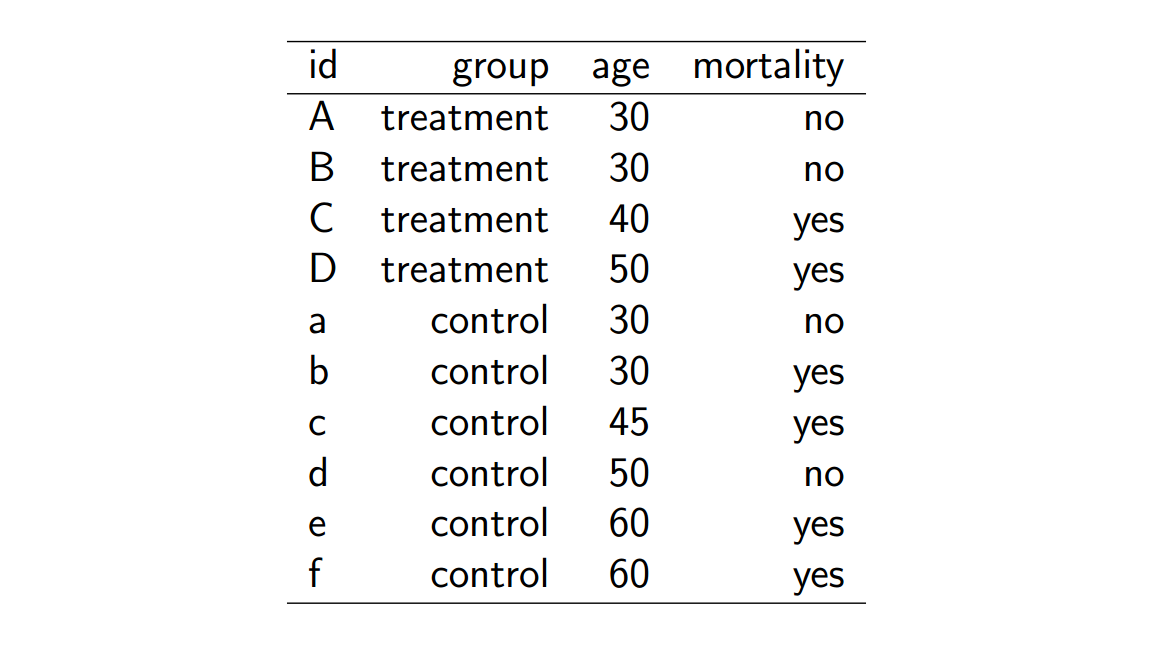
\includegraphics[width=0.7\linewidth]{fig/screenshot001}
	\caption{Conditional Contingency Table}
	\label{fig:screenshot001}
\end{figure}

The sample odd ratio is 
\[\hat{\theta} = \frac{\frac{\pi_1}{1 - \pi_1}}{\frac{\pi_2}{1 - \pi_2}} = \frac{\frac{n_{11}}{n_{12}}}{\frac{n_{21}}{n_{22}}} = \frac{n_{11}n_{22}}{n_{12}n_{21}}\]

\subsection{Unconditional Design}
Let $\pi_{ij}$ denote the true unknown joint probability of falling into the $ij$-th cell, $i=1,2$, $j=1,2$. The contingency table is as follows.

\begin{figure}[H]
	\centering
	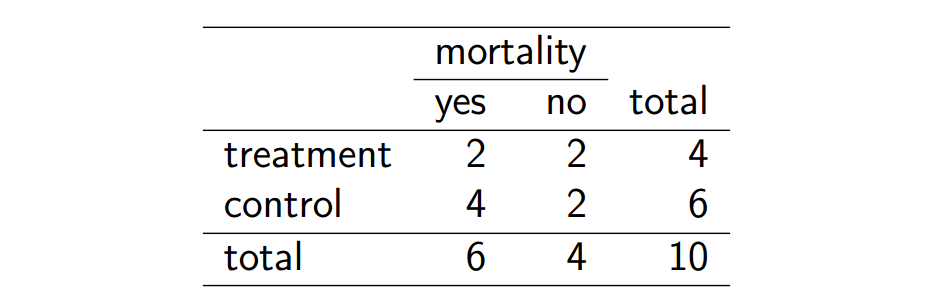
\includegraphics[width=0.7\linewidth]{fig/screenshot002}
	\caption{Unconditional Contingency Table}
	\label{fig:screenshot002}
\end{figure}

In the table, 
\begin{itemize}
	\item $\pi_{11} = \P(X = 1 \text{ and } Y = 1)$
	\item $\pi_{12} = \P(X = 1 \text{ and } Y = 1)$
	\item $\pi_{21} = \P(X = 0 \text{ and } Y = 1)$
	\item $\pi_{22} = \P(X = 0 \text{ and } Y = 0)$
\end{itemize}

The odd $\theta_1$ in the first row is 
\[\theta_1 = \frac{\P(Y = 1 | X = 1)}{P(Y = 0 | X = 1)} = \frac{\frac{\P(Y = 1, X = 1)}{\P(X = 1)}}{\frac{\P(Y = 0, X = 1)}{\P(X = 1)}} = \frac{\frac{\pi_{11}}{\pi_{11} + \pi_{12}}}{\frac{\pi_{12}}{\pi_{11} + \pi_{12}}} = \frac{\pi_{11}}{\pi_{12}}\]

The odd $\theta_2$ in the second row is 
\[\theta_2 = \frac{\P(Y = 1 | X = 0)}{P(Y = 0 | X = 0)} = \frac{\frac{\P(Y = 1, X = 0)}{\P(X = 0)}}{\frac{\P(Y = 0, X = 0)}{\P(X = 0)}} = \frac{\frac{\pi_{21}}{\pi_{21} + \pi_{22}}}{\frac{\pi_{22}}{\pi_{21} + \pi_{22}}} = \frac{\pi_{21}}{\pi_{22}}\]

Therefore, the population odd ratio is
\[\theta = \frac{\theta_1}{\theta_2} = \frac{\frac{\pi_{11}}{\pi_{12}}}{\frac{\pi_{21}}{\pi_{22}}} = \frac{\pi_{11}\pi_{22}}{\pi_{21}\pi_{22}}\]
Hence, the sample odd ratio is
\[\hat{\theta} = \frac{n_{11}n_{22}}{n_{21}n_{22}}\]

One may notice that the sample odd ratios are the same in two different studies.
\section{Odds Ratio of Matching Paired Data}
\subsection{Set-up}
Let $X$ be the treatment variable.
\begin{itemize}
	\item $X = 1$: treatment group
	\item $X = 0$: control group
\end{itemize}

Let $Y$ be the outcome variable. $Y = 1$ or $Y = 0$.

In the $j$-th pair, let $(Y_{j,t}, Y_{j, mc})$ be the outcome status of the treated individual and the matched individual in the control group.

The event status can be one of the four possibilities $(0, 0), (0, 1), (1, 0), (1, 1)$.

\begin{figure}[H]
	\centering
	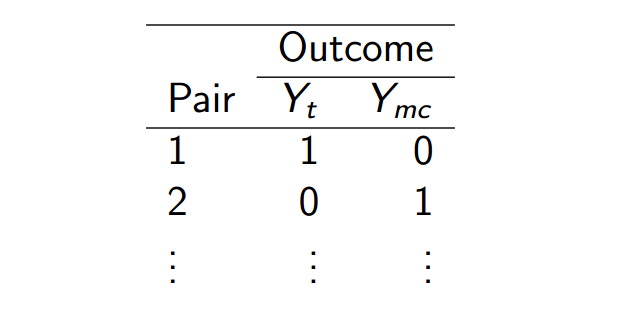
\includegraphics[width=0.5\linewidth]{fig/screenshot006}
	\caption{Paired Data List}
	\label{fig:screenshot006}
\end{figure}

The paired data can be represented into the contingency table.
\begin{figure}[H]
	\centering
	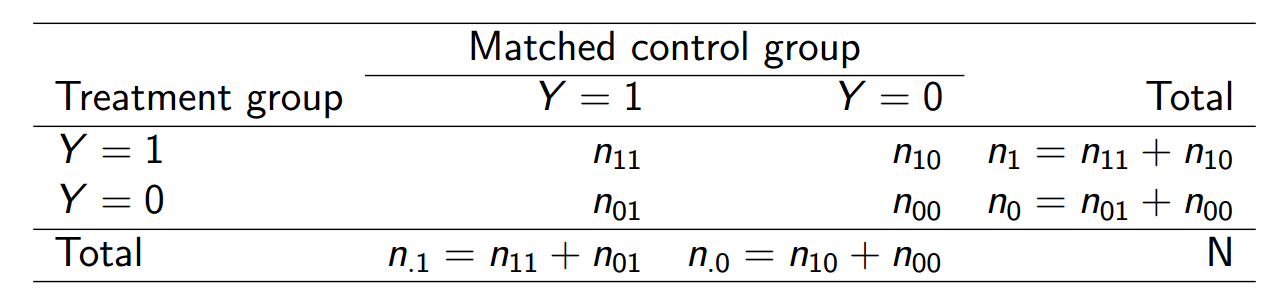
\includegraphics[width=0.7\linewidth]{fig/screenshot007}
	\caption{Contingency Table for Paired Data}
	\label{fig:screenshot007}
\end{figure}

Each frequency in the table represents number of pairs.
For instance, ``$n_{10}$'' means the number of pairs where the treated individuals have $Y= 1$ while the matched individual in the control group have $Y= 0$.

$N$ is the total number of pairs. $N = n_{11} + n_{10} + n_{01} + n_{00}$.

The proportion of $Y = 1$ 
\begin{itemize}
	\item in the treatment group is $(n_{11} + n_{10} / N)$.
	\item in the matched control group is $(n_{11} + n_{01} / N)$.
\end{itemize}

Hence, the difference of the proportions is $(n_{10} - n_{01}) / N$.

\subsection{Odds Ratio}
Use probabilities to represent paired groups.
\begin{figure}[H]
	\centering
	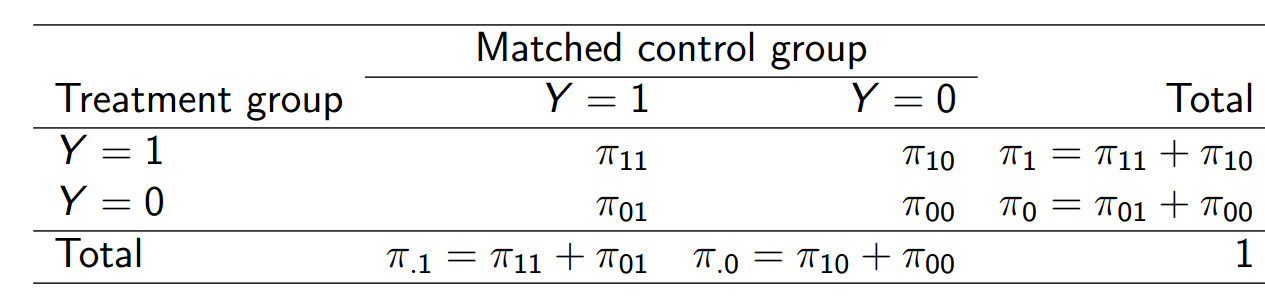
\includegraphics[width=0.7\linewidth]{fig/screenshot008}
	\caption{Probability in Contingency Table}
	\label{fig:screenshot008}
\end{figure}
In the table,
\begin{itemize}
	\item $\pi_{10} := \P(Y_{j,t} = 1, Y_{j, mc} = 0)$
	\item $\pi_{01} := \P(Y_{j,t} = 0, Y_{j, mc} = 1)$.
	\item $\pi_{1} := \P(Y_{j,t} = 1)$.
	\item $\pi_{.1} := \P(Y_{j, mc} = 1)$.
\end{itemize}

The odds ratio $\lambda = \pi_{10}/\pi_{01}$ measures the association between the outcome and the treatment.

An estimate of the odds ratio is $\hat{\lambda} = n_{10} / n_{01}$.

\subsection{Hypothesis Testing}
The null hypothesis is that the proportion of $Y = 1$ is the same in both treatment group and the matched control group.
\[H_0: \pi_{1} = \pi_{.1} \iff H_0: \pi_{10} = \pi_{01} \iff H_0: \lambda = 1\]

The alternative hypothesis is
\[H_1: \pi_1 \neq \pi_{.1}\]

The test statistic $T$ can be seen as approximately sampled from $\chi^2_1$ distribution for large sample.
\[T = \frac{(n_{10} - n_{01})^2}{n_{10} + n_{01}}\]

When consider continuity correction
\[T = \frac{(|n_{10} - n_{01}| - 1 )^2}{n_{10} + n_{01}}\]

Reject $H_0$ if $T > \chi_{\alpha,1}^2$.

\subsection{Example}
Johnson and Johnson (1972), in a study that was interested in
testing the theory that the tonsils protect the body against
invasion of the lymph nodes by a Hodgkin's disease virus,
obtained tonsillectomy data on 85 Hodgkin's cases and a sibling
of each case.

The data showed 41 tonsillectomies among the Hodgkin's cases
and 33 tonsillectomies among the siblings.
The pairing of a case with sibling means that the rates for the
two groups are not independent.

The pairing of a case with sibling means that the rates for the
two groups are not independent.
The pairing should be taken into account in the analysis in order
to achieve the best chance of detecting a departure from the null
hypothesis.
\[H_0: \text{Hodgkin's cases and their siblings have the same rates of
 tonsillectomy.}\]
The null hypothesis can be reduced to 
\[H_0: \text{The odds of tonsillectomy is the same.}\]

\begin{figure}[H]
	\centering
	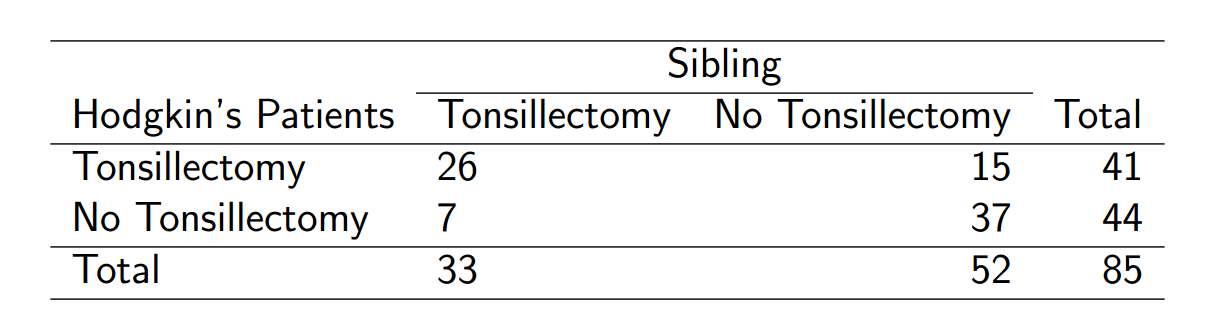
\includegraphics[width=0.7\linewidth]{fig/screenshot009}
	\caption{Contingency Table}
	\label{fig:screenshot009}
\end{figure}

\lstinputlisting[language=R]{code/l12-exp1.R}

\section{Fisher Exact Test}
Sir Ronald A. Fisher, the English statistician, has been called the
father of modern statistics.

\subsection{The Lady Tasting Tea}
A famous story, in Cambridge, England, in the late 1920is, that a colleague of Fisher's claimed that she
could tell, while drinking tea with milk, whether milk or tea was
poured into the cup first. 

An experiment was designed to test her claim.
\begin{itemize}
	\item 8 cups of tea were presented to her in a random order; 4 of these
	had milk poured first while the other 4 had tea poured first.
	\item She was told that there were 4 cups of each type.
\end{itemize}

Suppose we have the following data show the results of the experiment. 
\begin{figure}[H]
	\centering
	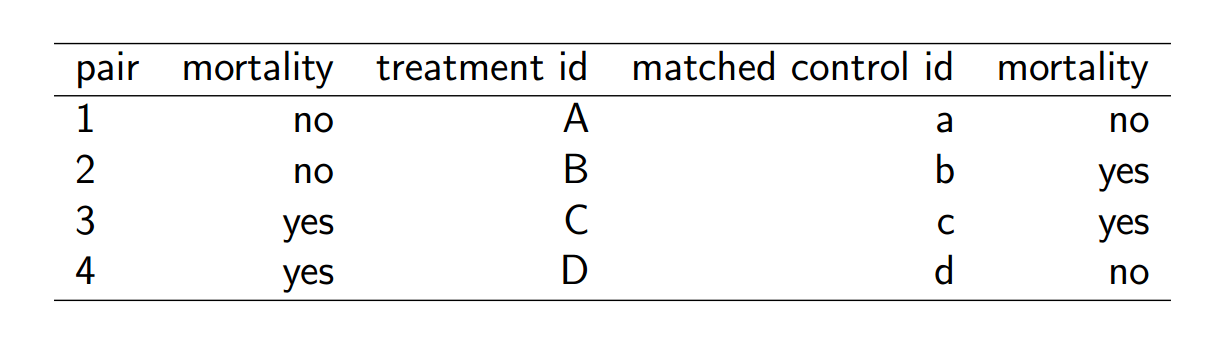
\includegraphics[width=0.7\linewidth]{fig/screenshot004}
	\caption{Contingenvy Table of Lady Tasting Tea}
	\label{fig:screenshot004}
\end{figure}

One can observe that she was right 3 out of 4 times on both types. Is this sufficient
evidence to support her claim of special power?

The contingency table has two difference comparing with the one we met.
\begin{itemize}
	\item The columns are fixed.
	\item The sample size is very small.
\end{itemize}

\subsection{Review: Hyper-geometric Distribution}
Suppose there are $m$ red balls and $n - m$ green balls. We randomly
pick $k$ balls without replacement. What is the probability that $z$ balls
are red?

Let $Z$ be the number of red balls.
\[\P(Z = z) = \frac{{m \choose z} {n-m \choose k - z}}{{n \choose k}}, z = 0, 1, \cdots, k.\]

Here we assume that
\begin{itemize}
	\item $z \le k$
	\item $z \le m$
	\item $k - z \le n - m$
\end{itemize}

\subsubsection{Example}

Suppose we have the following contingency table, in other words, $m = 6$, $n - m = 19$, $n = 25$. Also, $k = 10$ and $z = 1$. 
\begin{figure}[H]
	\centering
	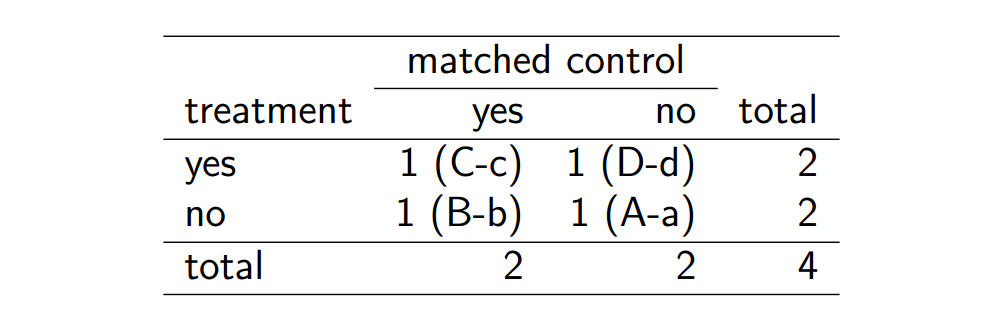
\includegraphics[width=0.7\linewidth]{fig/screenshot005}
	\caption{Hyper-geometric Distribution Example}
	\label{fig:screenshot005}
\end{figure}

We have
\[\P(Z = 1) = \frac{{6 \choose 1}{19 \choose 9}}{{25 \choose 10}}\]

The pdf of hyper-geometric distribution in R is as follows.
\begin{lstlisting}[language=R]
choose(6,1)*choose(19,9)/choose(25,10)
dhyper(x=1, m=6, 19, k=10)
\end{lstlisting}
\subsection{Fisher Exact Test}
Applying the hyper-geometric distribution, conditional on 4 guesses of having milk added first, the probability of
3 correct guesses is
\[\P(Z = 3) = \frac{{4 \choose 3}{4 \choose 4 - 3}}{{8 \choose 4}} = 0.229\]

So if the lady cannot tell the difference between two types of mix, there is still $22.9\%$ of probability for her to have 3 correct guesses by chance. Then how to exam her claim? Hypothesis Testing. To be more specific, Fisher Exact Test.

\subsection{Exact Inference for Small Samples}
The setup of Fisher Exact Test can be represented by the following contingency table.

\begin{figure}[H]
	\centering
	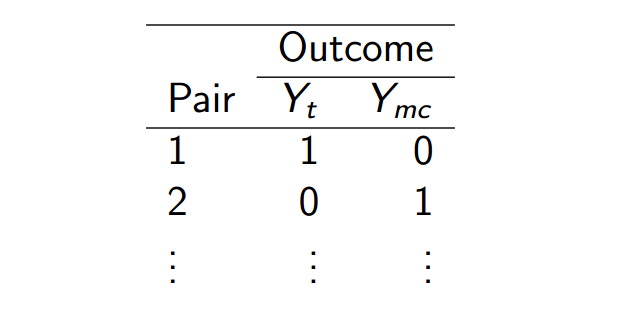
\includegraphics[width=0.7\linewidth]{fig/screenshot006}
	\caption{Contingency Table of Fisher Exact Test}
	\label{fig:screenshot006}
\end{figure}

In the table, $n_1$, $n$, and $n_{.1}$ are fixed. We can infer that $n_{.2} = n - n_{.1}$. $n_{11}$ is the observed random variable.

Fisher's exact test is based on the conditional distribution of $n_{11}$ given $n_1$, $n$, and $n_{.1}$. Given, $z \le \min\{n_1, n_{.1}\}$, and $n_{.1} - z \le n_2$,
\[\P(n_{11} = z) = \frac{{n_1 \choose z} {n_2 \choose n_{.1} - z}}{{n \choose n_{.1}}}.\]

Recall that the $p$-value is calculated by the sum of all event which are equal or rarer than the observed event.

Note that the estimated odd ratio is different from the calculation we have been using. It is because that the experiment design is different with the ones we have. The estimation of odd ratio can be found in R's fisher test manual.
\lstinputlisting[language=R]{code/l10-fisher-exact.R}

\section{Example}
A study concerns the approval ratings of a prime minister in two
surveys.
In the first survey, ratings were obtained on 1600 citizens and
then in a second survey, six months later, the same citizens were
resurveyed.

\begin{itemize}
	\item In the 1st survey, 944 indicated approval of the Prime Minister's
	performance in office.
	\item In the 2nd survey, 880 indicated approval.
\end{itemize}

There each subject has two observation. So that we have 1600 pairs of data out of 1600 people.

\begin{figure}[H]
	\centering
	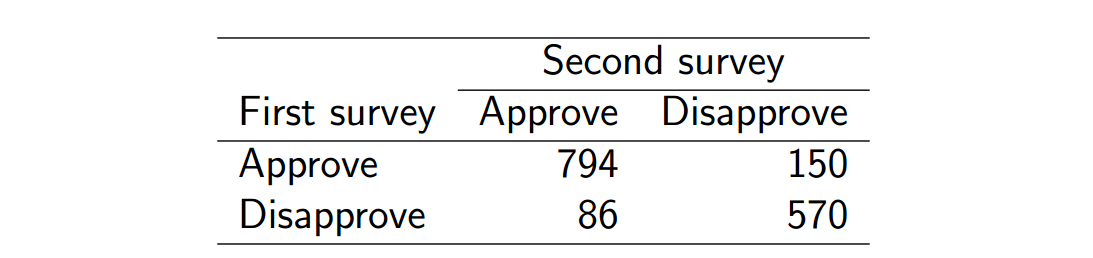
\includegraphics[width=0.7\linewidth]{fig/screenshot010}
	\caption{Contingency Table}
	\label{fig:screenshot010}
\end{figure}

The null hypothesis is 
\[H_0: \text{the approval rate does not change.}\]
It can be reduced to
\[H_0: \text{the odds of approval does not change.}\]
It means that the probability of going from approval to disapproval is the
same as the probability of going from disapproval to approval.

In the following code, we identify that 4 more percentage of people going from approval to disapproval. McNemar test tells us that it is significant.

\lstinputlisting[language=R]{code/l12-exp4.R}

kappa test focus on the agreement while the McNemar Test focus on the disagreement.

\lstinputlisting[language=R]{code/l12-exp5.R}
\end{document}
